\documentclass[
	aspectratio=169, % default is 43
	8pt, % font size, default is 11pt
	%handout, % handout mode without animations, comment out to add animations
	nosectionframes, % disable automatic frames at the begin of each section (default: sectiontitleslides in beamer mode and sectionoverviews in handout mode)
	%sectiontitleslides, % enable an automatic section title slide at the begin of each section
	%sectionoverviews, % enable an automatic section overview at the begin of each section
	%uniqueslidenumber, % will uniquely identify pages with overlays by a little suffix
	%darkmode, % switch to dark mode
]{beamer}

\usepackage{beamerthemeuulm} % use the inofficial uulm beamer theme
\setfaculty{infIngPsy} % set the color scheme for your faculty here [med/infIngPsy/math/nat]

\usepackage{twemojis}

\usepackage{listings}
\usepackage{tikz}
\usepackage{qrcode}
\usetikzlibrary{positioning,fit,backgrounds,arrows,shapes}
\usetikzlibrary{overlay-beamer-styles}
\lstdefinelanguage{uvlfull}{
    basicstyle=\linespread{0.77}\selectfont,
	keywords = {alternative,or,optional,mandatory,features,constraints, cardinality, Real, Boolean, Integer, String, imports, as,include},
    otherkeywords={|,&,[,], ==, =>, <, \{,\}},
	morecomment=[l]{//},
	commentstyle=\itshape\color{purple!40!black},
    keywordstyle=\ttfamily\color{magenta},
    tabsize=4,
    columns=fullflexible
}

%\institutelogo{sp} % set the institute logo
%\universitylogo{uulm} % set a new university logo
%\clearuniversitylogo % clear existing university logo
%\clearinstitutelogo % clear existing institute logo
%\uulmlogos{sp,uulm} % freely configure multiple logos (overwrites any other logo setting)
\uulmlogos{} % include softvare working group logo

%\usepackage[ngerman]{babel} % use this line for slides in German

%\setmycolumnsdefault{keep} % change the default for 'mycolumns' environment (e.g., 'keep' to animate all column environments per default)

%\includeonlyframes{current} % default mechanism of beamer to include only labeled frames, can be used for debugging or drafting

\title[UVL: Current State]{Universal Variability Language: Current State} % short title is used for the slide footer but optional
\subtitle[MODEVAR'25]{MODEVAR'25} % subtitles are optional at all
\author[Chico Sundermann]{Contributions by many great people, Talk by Sebastian Krieter} % short author title is used for the slide footer but optional
\date{03.02.2024} % use a particular date here if needed

\newcommand{\inlinesubtitle}[1]{\textcolor{gray!60}{~{}~#1}}

\begin{document}

\maketitle[bern-modevar] % title page with default picture

\section{Universal Variability Language}

\begin{frame}
	\frametitle{\insertsection}
	\begin{columns}
		\begin{column}{0.49\textwidth}
			\begin{itemize}
				\item Community Effort within MODEVAR initiative
				\item Textual format for variability models
				\item Simplify exchange
				\item<2-> Simple core language
                \begin{itemize}
                    \item Boolean constraints \& features
                \end{itemize}
                \item<2-> Extensions for complex expressions
                \item<3-> \textbf{Let's take a look!}
			\end{itemize}
		\end{column}

		\begin{column}{0.49\textwidth}
			\begin{tikzpicture}
				\node[draw] at (0,0) {\lstinputlisting[language=uvlfull]{snippets/02-basicattributed.uvl}};
			\end{tikzpicture}
		\end{column}
	\end{columns}
\end{frame}

\section{Language Levels}

\begin{frame}{\insertsection \inlinesubtitle{Tradeoff}}
    \begin{figure}
        \begin{tikzpicture}
            \node (simple) at (0,0) {
\includegraphics[width=3cm]{pics/Knife.png}};
            \node[below=1cm of simple, align=left] {\textbf{+} Simple \\ \textbf{+} Easy to understand \\ \textbf{--} Limited applicability};
            \node[right=2cm of simple] (vs) {\huge VS};
            \node[right=2cm of vs] (complex) {
\includegraphics[width=4cm]{pics/Swiss.png}};
            \node[below=1cm of complex, align=left] {\textbf{+} Covers more use cases \\ \textbf{--} Complex \\ \textbf{--} Harder to understand};
        \end{tikzpicture}
    \end{figure}
\end{frame}

\begin{frame}{\insertsection \inlinesubtitle{Overview}}
	\begin{columns}[t]
		\begin{column}{0.3\textwidth}
            \textbf{Boolean}
			\begin{itemize}
                    \item Boolean constraints \& features
                    \item Feature attributes for information
			\end{itemize}
               \begin{tikzpicture}
				\node[draw,scale=0.5] at (0,0) {\lstinputlisting[language=uvlfull]{snippets/02-basicattributed.uvl}};
			\end{tikzpicture}
		\end{column}
  		\begin{column}{0.3\textwidth}
            \textbf{Arithmetic}
			\begin{itemize}
                    \item Numeric constraints over feature attributes
                    \item Expressions such as ==
			\end{itemize}
   			\begin{tikzpicture}
				\node[draw,scale=0.5] at (0,0) {\lstinputlisting[language=uvlfull]{snippets/03-arithmetic.uvl}};
			\end{tikzpicture}
		\end{column}
  		\begin{column}{0.3\textwidth}
            \textbf{Type}
			\begin{itemize}
                    \item Feature types
                    \item Constraints over typed features
			\end{itemize}
   			\begin{tikzpicture}
				\node[draw,scale=0.5] at (0,0) {\lstinputlisting[language=uvlfull]{snippets/04-type.uvl}};
			\end{tikzpicture}
		\end{column}
	\end{columns}
\end{frame}

\begin{frame}{\insertsection \inlinesubtitle{The Pain}}
    \begin{figure}
        \centering
        \begin{tikzpicture}
            \node[draw] (fide) at (0,0) {
\includegraphics[width=2cm]{pics/featureIDE.png}};
            \node[left=3cm of fide] (fama)  {
\includegraphics[width=2cm]{pics/FAMA.png}};
            \node[right=3cm of fide] (familiar)  {
\includegraphics[width=2cm]{pics/Familiar.png}};
        
            \node[draw, above = 1cm of fide,scale=0.6] (fideuvl) {\lstinputlisting[language=uvlfull]{snippets/02-basicattributed.uvl}};
            \node[draw, above = 1cm of fama,scale=0.6] (famauvl) {\lstinputlisting[language=uvlfull]{snippets/03-arithmetic.uvl}};
            \node[draw, above = 1cm of familiar,scale=0.6]  (familiaruvl) {\lstinputlisting[language=uvlfull]{snippets/04-type.uvl}};

            \uncover<2> {
                \draw[thick, red, -latex] (fide.north) to (famauvl.south);
                \draw[thick, red, -latex] (fide.north) to (familiaruvl.south);
            }
        \end{tikzpicture}
    \end{figure}
\end{frame}

\begin{frame}{\insertsection \inlinesubtitle{How to Resolve?}}
    \begin{figure}
        \centering
        \begin{tikzpicture}
            \node[draw] (fide) at (0,0) {
\includegraphics[width=2cm]{pics/featureIDE.png}};


            \uncover<2->{
    			\node[above = 1cm of fide, draw=gray, fill=gray!10] (after) {\lstinputlisting[language=uvlfull,basicstyle=\small]{snippets/smtbasic-Boolean.uvl}};
            }
            
            \node[left = 3cm of after, draw=gray, fill=gray!10] (before) {\lstinputlisting[language=uvlfull,basicstyle=\small]{snippets/smtbasic.uvl}};

            \uncover<1>{
                \draw[-latex,red] (before.south) -- node[above,align=center] {\textbf{Invalid Input}} (fide.north);
            }
            
            \uncover<2->{
                \draw[-latex] (before) -- node[above,align=center] {\textbf{Conversion} \\ \textbf{UVLParser}} (after);
            }

            \uncover<3>{
                \draw[-latex] (after.south) -- node[right,align=center] {\textbf{Valid Input}} (fide.north);
            }

        \end{tikzpicture}
    \end{figure}
\end{frame}



\begin{frame}[plain]
	\begin{figure}
		\scalebox{1.7}{
			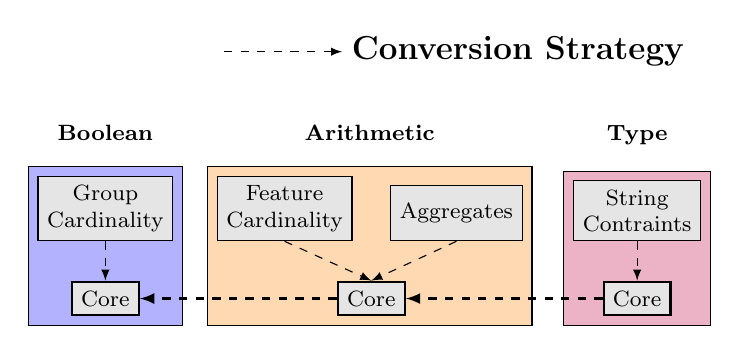
\begin{tikzpicture}

				\tikzstyle{every node}=[font=\footnotesize]
				\node[rectangle,draw=black,fill=gray!20, thick] (satcore) at (0,0) {Core};
				\node[rectangle,draw=black,fill=gray!20, above= 0.5cm of satcore,align=center, minimum height=0.7cm] (group cardinality) {Group \\ Cardinality};
				\draw[dashed,-latex] (group cardinality.south) -- (satcore.north);


				\begin{pgfonlayer}{background}
					\node [fill=blue!30,draw=black,fit=(satcore) (group cardinality)] (satbox) {};
				\end{pgfonlayer}
				\node[above=0.2cm of satbox] {\textbf{Boolean}};


				\node[rectangle,draw=black,fill=gray!20, thick, right = 2.5cm of satcore] (smtcore) {Core};
				\node[rectangle,draw=black,fill=gray!20, above left= 0.5cm and -0.2cm of smtcore,minimum height=0.7cm,align=center] (featurecardinality) {Feature \\ Cardinality};
				\node[rectangle,draw=black,fill=gray!20, above right= 0.5cm and -0.2cm of smtcore,minimum height=0.7cm] (aggregates) {Aggregates};
				\draw[dashed,-latex] (featurecardinality.south) -- (smtcore.north);
				\draw[dashed,-latex] (aggregates.south) -- (smtcore.north);
				\draw[dashed,-latex,thick] (smtcore.west) -- (satcore.east);



				\begin{pgfonlayer}{background}
					\node [fill=orange!30,draw=black,fit=(smtcore) (featurecardinality) (aggregates)] (smtbox) {};
				\end{pgfonlayer}
				\node[above=0.2cm of smtbox] (arithmeticlabel) {\textbf{Arithmetic}};

					\node[above right= 0.5cm and -1.3cm of arithmeticlabel] (conversionlabel) {\large \textbf{Conversion Strategy}};
					\draw[dashed,-latex] (conversionlabel.west)++(-1.5,0) -- (conversionlabel.west);



				\node[rectangle,draw=black,fill=gray!20, thick, right = 2.5cm of smtcore] (typecore) {Core};
				\node[rectangle,draw=black,fill=gray!20, above= 0.5cm of typecore,align=center, minimum height=0.7cm] (stringconstraints) {String \\ Contraints};


				\draw[dashed,-latex] (stringconstraints.south) -- (typecore.north);
				\draw[dashed,-latex,thick] (typecore.west) -- (smtcore.east);


				\begin{pgfonlayer}{background}
					\node [fill=purple!30,draw=black,fit=(typecore) (stringconstraints)] (typebox) {};
				\end{pgfonlayer}
				\node[above=0.2cm of typebox] {\textbf{Type}};

			\end{tikzpicture}
		}
		\caption{Language Levels in UVL}
		\label{figure:languagelevels}
	\end{figure}

\end{frame}

\section{What Can We Do?}

\newcommand{\new}[1]{\twemoji{rolled-up newspaper} \textbf{\textcolor{green}{#1}}}


\begin{frame}{\insertsection \inlinesubtitle{Parsing}}
\vspace{0.4cm}
    \begin{columns}[t]
		\begin{column}{0.49\textwidth}
			\textbf{UVL-Parser}
            \begin{itemize}
                \item ANTLR-based
                \begin{itemize}
                    \item Parser generator for many languages
                \end{itemize}
                \item Currently supported: Java, Python, \new{JavaScript}
            \end{itemize}
		\end{column}%
		\begin{column}{0.49\textwidth}
           \begin{figure}
                \centering
                
\includegraphics[width=5cm]{pics/qr/uvl-parser.pdf}
                \caption{UVL-Parser GitHub Repo}
            \end{figure}
		\end{column}
	\end{columns}
\end{frame}

\begin{frame}{\insertsection \inlinesubtitle{Editing}}
    	\begin{columns}[t]
		\begin{column}{0.3\textwidth}
            \textbf{UVLS}
			\begin{itemize}
                    \item Textual editing
                    \item Language Server for UVL
                    \item Extension VSCode
                    \item Support for full language
			\end{itemize}
            \begin{figure}
                \centering
                
\includegraphics[width=3cm]{pics/qr/uvls.pdf}
                \caption{UVLS GitHub Repo}
            \end{figure}

		\end{column}
  		\begin{column}{0.3\textwidth}
            \textbf{UVL-Playground}
			\begin{itemize}
                    \item Web-based
                    \item Internally uses UVLS
                    \item Includes small UVL tutorial
                    \invisible{\item d}
			\end{itemize}
   			            \begin{figure}
                \centering
                
\includegraphics[width=3cm]{pics/qr/uvlplayground.pdf}
                \caption{UVL Playground}
            \end{figure}

		\end{column}
  		\begin{column}{0.3\textwidth}
            \textbf{FeatureIDE}
			\begin{itemize}
                    \item Graphical Editing
                    \item Limited to Boolean UVL
                    \invisible{\item d}
                    \invisible{\item d}
			\end{itemize}
   			            \begin{figure}
                \centering
                
\includegraphics[width=3cm]{pics/qr/featureide.pdf}
                \caption{FeatureIDE Git Repo}
            \end{figure}

		\end{column}
	\end{columns}
\end{frame}

\begin{frame}{\insertsection \inlinesubtitle{Conversion}}
    	\begin{columns}
		\begin{column}{0.49\textwidth}
			\textbf{TraVarT}
            \begin{itemize}
                \item Convert between variability languages
                \begin{itemize}
                    \item Feature models
                    \item Decision models
                    \item OVM
                \end{itemize}
            \end{itemize}
            \begin{figure}
                \centering
                
\includegraphics[width=3cm]{pics/qr/travart.pdf}
                \caption{TraVarT GitHub Repo}
            \end{figure}

		\end{column}

		\begin{column}{0.49\textwidth}
			\textbf{UVL Parser Conversions}
   \begin{itemize}
       \item Convert between language levels
       \item Included in Java Parser (Meta Model)
       \invisible{\item d}
       \invisible{\item d}
   \end{itemize}
               \begin{figure}
                \centering
                
\includegraphics[width=3cm]{pics/qr/metamodel.pdf}
                \caption{Meta Model GitHub Repo}
            \end{figure}
   
		\end{column}
	\end{columns}
\end{frame}


\begin{frame}{\insertsection \inlinesubtitle{Analysis}}
    \vspace{0.4cm}
    \begin{columns}[t]
		\begin{column}{0.49\textwidth}
			\textbf{FLAMA}
            \begin{itemize}
                \item Python-based
                \item Common analyses: SAT, counting
                \item Reasoning engines: SAT, SMT, BDDs
            \end{itemize}
            \begin{figure}
                \centering
                
\includegraphics[width=0.5\columnwidth]{pics/qr/flama.pdf}
                
                FLAMA GitHub Repo
            \end{figure}
		\end{column}%
		\begin{column}{0.49\textwidth}
            \new{FeatJar}
            \begin{itemize}
                \item Java-based
                \item \dots
                \item ...
            \end{itemize}
            \begin{figure}
                \centering
                
\includegraphics[width=0.5\columnwidth]{pics/qr/featjar.pdf}
                
                FeatJar GitHub Repo
            \end{figure}
		\end{column}
	\end{columns}
\end{frame}

\begin{frame}{\insertsection \inlinesubtitle{Collections}}
    \vspace{0.4cm}
    \begin{columns}[t]
		\begin{column}{0.3\textwidth}
			\textbf{UVL-models}
            \begin{itemize}
                \item Small collection
                \item Translated from various variability languages
                \item Limited to boolean
            \end{itemize}
            \begin{figure}
                \centering
                
\includegraphics[width=3cm]{pics/qr/collection.pdf}
                \caption{UVL-Models GitHub Repo}
            \end{figure}
		\end{column}%
		\begin{column}{0.3\textwidth}
            \new{Feature-Model Benchmark}
            \begin{itemize}
                \item GitHub Repository
                \item $>2,500$ models with at least 100 features
                \item UVL, DIMACS
            \end{itemize}
            \begin{figure}
                \centering
                
\includegraphics[width=3cm]{pics/qr/benchmark.pdf}
                \caption{Benchmark GitHub Repo}
            \end{figure}
		\end{column}
        \begin{column}{0.3\textwidth}
            \new{UVLHub}
            \begin{itemize}
                \item Share UVL models
                \item Automated analysis for each upload
                \item $>1,500$ models available  
            \end{itemize}
            \begin{figure}
                \centering
                
\includegraphics[width=3cm]{pics/qr/uvlhub.pdf}
                \caption{UVLHub GitHub Repo}
            \end{figure}
        \end{column}
	\end{columns}
\end{frame}


\begin{frame}
	\frametitle{\inserttitle}

	\leftandright{
		\begin{itemize}
			\item Language as community effort
            \item Extensible language design
            \item Language Features
            \begin{itemize}
                \item Language levels
                \item Conversion strategies
                \item Import mechanism
            \end{itemize}
            \item Available tool support:
            \begin{itemize}
                \item Parsing
                \item Editing
                \item Conversion
                \item Analysis
                \item Collections
            \end{itemize}
            \item \textbf{What do we need?}
		\end{itemize}
	}{
		\begin{figure}
			\centering
			
\includegraphics[width=0.7\columnwidth]{pics/qr/homepage.pdf}
			\caption{https://universal-variability-language.github.io}
		\end{figure}

	}

\end{frame}


\contentoverview

\end{document}